% !TEX root = ../main.tex
\paragraph{High Threshold Cherenkov Counter (HTCC)}
    \begin{wrapfigure}{l}{0.50\textwidth}
        \centering\frame{
        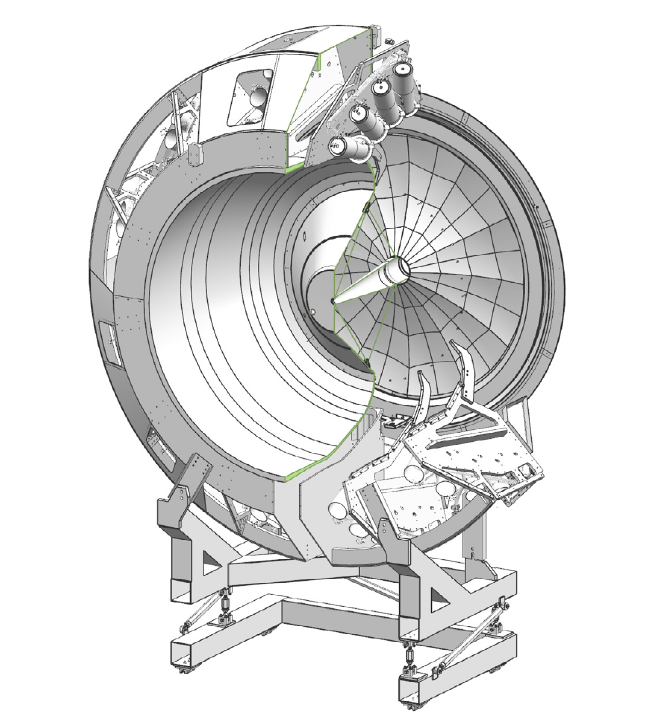
\includegraphics[width=\linewidth]{211htcc.png}}
        \caption[HTCC]{Render of the High Threshold Cherenkov Counter.
        The container spans a diameter of about 4.5 m. The mirror is seen at the downstream end to the right.
        The Photomultiplier Tubes (PMTs) are mounted in 12 sectors and in groups of 4 at the outer perimeter of the container.
        Light collection uses additional Winston cones and 5-in PMTs with quartz windows.
        Source: \hyperlink{jlab.org/physics/hall-b/clas12}{CLAS12 wiki}.}
        \label{fig::11.211::htcc}
    \end{wrapfigure}

    The HTCC is specifically designed to separate electrons and positrons with momenta below 4.9 GeV from other charged particles.
    It achieves this through its capability for electron/positron identification, which provides high rejection of charged pions and low background noise.
    This is crucial for reliably identifying scattered electrons in an environment with a dense electromagnetic background.

    The HTCC is positioned downstream of the target and is fitted in between magnets, upstream of the forward tracking detectors.
    It ensures full azimuthal coverage, meaning it can detect particles emitted from any direction around its circumference.
    In terms of the polar angle, it spans from $5\degree$ to $35\degree$, covering a specific range of particle emission angles.
    Importantly, it has no blind areas in its complete solid angle coverage, meaning there are no regions where particles cannot be detected.

    Operating in dry CO2 gas at 1 atm pressure, the HTCC consists of a multi-focal mirror composed of 48 elliptical mirror facets.
    This mirror design enables the focusing of Cherenkov light produced by charged particles passing through the detector.
    The focused light is then detected by 48 PMTs, with each PMT featuring a quartz window of 125 mm in diameter.

    The PMTs are positioned within a magnetic field of up to $3.5\cdot 10^{-3}$ T, which is oriented along the axes of the phototubes.
    To minimize the impact of the magnetic field on the PMTs, they are surrounded along their lengths by a multi-layer magnetic shield.
    This shield includes active compensation coils, which further help in shielding the PMTs from the effects of the magnetic field.

    To minimize the effects of multiple scattering and its impact on the momentum analysis of charged tracks in the torus field, the HTCC mirror system is constructed using a backing structure made of low-density composite material.
    This choice of material helps to reduce the scattering of particles passing through the HTCC, thereby improving the accuracy of momentum measurements.

    Since the HTCC is located in front of the momentum analyzing torus magnet, it is important to minimize the presence of materials in the path of charged particles, except for the radiator gas.
    This is done to prevent interactions and disturbances that could affect the accuracy of momentum analysis.
    The HTCC is designed with this consideration in mind.

    In the HTCC, the density of solid material encountered by charged particles passing through its volume is approximately $135~\text{mg/cm}^2$.
    This low-density configuration ensures that the material contribution to multiple scattering is minimised, allowing for more precise momentum measurements of charged tracks.

    The HTCC also serves the purpose of generating a fast signal that can be used as a trigger for scattered electrons.
    This signal is utilised to identify and select scattered electrons for further analysis.

    In conjunction with the energy deposited in the electromagnetic calorimeters, the HTCC plays a role in the identification of electrons with specific energies.
    By combining the information from the HTCC and the electromagnetic calorimeters, the experiment can accurately identify electrons of interest based on their energy deposition patterns.

    A visual representation of the HTCC can be seen in Figure \ref{fig::11.211::htcc}, which provides a cut view of the detector and its components.

    Overall, the HTCC plays a crucial role in electron/positron identification by using a multi-focal mirror, PMTs, and a magnetic field setup.
    These components work together to ensure efficient detection and separation of electrons and positrons from other charged particles in a high-energy physics experiment environment.
